\documentclass[a4paper,titlepage]{article}
\usepackage[italian]{babel}
\usepackage{graphicx}
\usepackage{float}
\usepackage[utf8]{inputenc}
\usepackage{amsmath}
\usepackage[noend]{algorithmic}
\usepackage{color}
\usepackage{floatpag}
\usepackage{listings}
\usepackage{textcomp}
\usepackage{caption}
\usepackage{afterpage}
\usepackage{titling}
\usepackage{titlesec}
\usepackage{pbox}
\usepackage{tabularx}
\linespread{1.3}
\newcommand{\subtitle}[1]{%
  \posttitle{%
    \par\end{center}
    \begin{center}\large#1\end{center}
    \vskip0.5em}%
}
\renewcommand{\lstlistingname}{Code}

\definecolor{listinggray}{gray}{0.9}
\definecolor{lbcolor}{rgb}{0.9,0.9,0.9}
\lstset{
backgroundcolor=\color{lbcolor},
		tabsize=3,    
		linewidth=13.5cm,
		language=MATLAB,
        basicstyle=\scriptsize,
        upquote=true,
        aboveskip={1.5\baselineskip},
        columns=fixed,
        showstringspaces=false,
        extendedchars=false,
        breaklines=true,
        prebreak = \raisebox{0ex}[0ex][0ex]{\ensuremath{\hookleftarrow}},
        frame=single,
        numbers=left,
        showtabs=false,
        showspaces=false,
        showstringspaces=false,
        identifierstyle=\ttfamily,
        keywordstyle=\color[rgb]{0,0,1},
        commentstyle=\color[rgb]{0.026,0.112,0.095},
        stringstyle=\color[rgb]{0.627,0.126,0.941},
        numberstyle=\color[rgb]{0.205, 0.142, 0.73}
}
\lstset{
    backgroundcolor=\color{lbcolor},
    tabsize=2,
  language=sh,
  captionpos=b,
  tabsize=3,
  frame=lines,
  numbers=left,
  numberstyle=\tiny,
  numbersep=5pt,
  breaklines=true,
  showstringspaces=false,
  basicstyle=\footnotesize,
%  identifierstyle=\color{magenta},
  keywordstyle=\color[rgb]{0,0,1},
  commentstyle=\color{green},
  stringstyle=\color{red}
  }

  
\titlespacing*{\subsubsection}{0pt}{1.1\baselineskip}{\baselineskip}

\begin{document}
\pagenumbering{gobble}
%topmatter
\title{Assignment 1 IM - HL7 Message Parsing}
\author{Gerardo Vitagliano - 2017214620 \\ Martin Schlegel - 2017190694 }
\date{\vspace{-5ex}}
\vfill
\maketitle
\clearpage
\section{HL7 Message}
The message consists of 13 segments:
\begin{enumerate}
  \item Message Header (MSH): Here we define the receiving and sending applications/ units, the time, the message type and the version of HL7. We use version 2.7, because it is the newest one and includes the NextOfKin-segment. The message type is defined as ORU\textasciicircum R01 to declare it is a unsolicited observation result.
  \item Patient Data (PID): In this segment we store all patient directed data, like the name, address and given contact details.
  \item NextOfKin (NK1): These segments stores the information of the responsible person for the patient. In this case here are stored values related to the patients wife.
  \item Observation Result (OBR): We decided to use two different OBR- Segments to save the different kinds of data (numeric and time series). The first OBR saves the numeric data in the following OBX segments.
  \item 7 Observation Segments (OBX's): These segments are storing the specific numeric values, like the height, weight of the patient in different OBX segments. To show the connection to the previous defined OBR they have an ongoing index.
  \item Observation Result (OBR): The second OBR stores the time series values of the Photoplethysmography (PPG) we took during the class.
  \item Observation Segments (OBX): Here are the PPG values. The different values are seperated by '\textasciicircum'.
\end{enumerate}

\section{Parser}

The implemented parser takes into account the structure of the message according to the HL7 standard 2.7. Due to the task requested, the parser does no full check over HL7 2.7 syntax, but instead takes into account only the specific case of a ORU\textasciicircum R01 message.
Moreover, it implements a logic to check the correct use of segments, without further analyzing fields and subfields.
In this section the MATLAB script code will be analyzed one chunk at a time, in order to explain in detail its behaviour.\\
The very first lines of code have the task of importing the message in the MATLAB environment and extract the relevant information to obtain
a structured data containing the message. The input file is imported with the use of textscan: since the segments in the HL7 message are separated by a new line, the "Delimiter" option can be used to separate different text lines. This function returns a cell structure with just one cell, containing inside an Nx1 string matrix in which every row element corresponds to one of the N segment of the original message.
This matrix is stored in the temporary variable 'res'.
\begin{lstlisting}[caption=Message import]
[fileID,msg] = fopen('message.hl7');
inp = textscan(fileID,'%s','Delimiter','\n');
res=vertcat(inp{1,1});
fclose(fileID);
\end{lstlisting}

Right after the segments are imported, the next task is separating fields contained in a segment. The desired output is a NxM matrix, where M is the maximum number of fields contained in a segment received.
Because M is not known in advance, since segments can have a different and not fixed number of fields, there is the need of two nested for loops. The outer one will retrieve the fields for each segment, and transpose them in order to get a row vector, while the inner one, in case the number of fields of current segment is greater than the one in the previous ones, has the task to "pad" all the previous rows to fit them in the new dimensions of the matrix.
At the end of this code, the variable 'field' will be an NxM string matrix, in which the (i,j) element is the j-th field of the i-th segment.
\begin{lstlisting}[caption=Message formatting]
columns=1;
rows=length(res);
 for i=1:rows
    temp = strread(res{i,1},'%s','delimiter','|')'; %The output is transposed so to get every segment on a row
    if length(temp)>columns %Columns store the maximum number of fields found
        for j=1:i           %if a new segment has more field than the previous, the previous are padded with '\p'
            fields(j,columns+1:length(temp))={'\p'};  %to pad, the old value of columns is used until the new one
        end
         columns=length(temp);
    end
    fields(i,1:length(temp))=temp;
 end
     
end
\end{lstlisting}

After the message is properly imported, the code follows checking the validity of the segments. The very first lines check that the proper header, MSH, and that the second is the Patient Identification. In fact, according to HL7 2.7 syntax, these two segments are mandatory, and in this order.

\begin{lstlisting}[caption=Validity of MSH and PID segments]
if ~strcmp(fields{1,1},'MSH')
    disp('First segment is not MSH - invalid syntax');
    return
end
if ~strcmp(fields{2,1},'PID')
    disp('Second segment is not Patient ID - invalid syntax');
    return
end
\end{lstlisting}

The following check is to be sure the message sent actually contains an OBR segment, since being a Observation Request this segment is mandatory.
However, given the possible flexibility in the message structure, there is no fixed position for an OBR segment: because of this a for loop is used to check all the segments. This loop starts from 3 since the two first fields, for the message to be valid, must be MSH and PID. In case at least one OBR segment is found, the variable validOBR is set to be true.
Since every OBR can one or more associated OBX segments, after finding one OBR a set of check is performed in order to validate the presence and the correct ordering of the IDs for eventual OBX segments.
The variable validOBX is at first set as true, since an OBX segment could not be present at all without this being an error, while is set to false in case an OBX segment is found with an invalid ID.
Additional checks are present in order to consider situations in which the message ends with an OBR segment, and thus preventing an out-of-bound exception while trying to access a row index in overflow for the 'fields' matrix.

\begin{lstlisting}[caption=Validity of OBR/OBX segments]
%There should be at least one OBR segment, if there are any 
validOBR=false;
validOBX=true;
for i=3:rows
    if strcmp(fields{i,1},'OBR')
        validOBR=true;
        if (i+1<rows)                        %check if the message does not end with an OBR segment
            if strcmp(fields{i+1,1},'OBX')
                if(1~=str2num(fields{i+1,2}))   %If the first OBX is not with ID 1
                    validOBX=false;
                    break
                end
                j=2;
                if(i+j<rows)                    %Check if the message ends with an OBX
                    while strcmp(fields{i+j,1},'OBX') %check if subsequent OBX have correct ID
                        if (j~=str2num(fields{i+j,2}))
                            validOBX=false;
                            break
                        end
                    j=j+1;    
                    end
                end
            end
        end
    end
end

if ~validOBR
    disp('There is not an OBR segment - invalid syntax');
    return
end

if ~validOBX
    disp('There is a problem with OBX segment indexes - invalid syntax');
    return
end
\end{lstlisting}

Finally, given the correctness of segment syntax, the value of the fields is retrieved for an output to the user.
This is done using the strsplit MATLAB function taking into account that values in fields are separated by the '\textasciicircum' character.
Given the formatting of the field matrix, the needed information is in fixed position: in fact even though some fields are not presents, these will result in empty cells of the matrix. This formatting was chosen rightly in order to guarantee ease of value retrieval. 
\begin{lstlisting}[caption=Information Retrieval]
name=strsplit(fields{2,6},'^');
height=fields{5,6};
heightMeasure=strsplit(fields{5,7},'^');

weight=fields{6,6};
weightMeasure=strsplit(fields{6,7},'^');

heartRate=fields{7,6};
heartMeasure=strsplit(fields{7,7},'^');

sysPre=fields{8,6};
sysMeasure=strsplit(fields{8,7},'^');

dyaPre=fields{9,6};
dyaMeasure=strsplit(fields{9,7},'^');
\end{lstlisting}

The last lines of code simply perform output of the information retrieved from the message.
\begin{lstlisting}[caption=Information Retrieval]
fprintf('Information about the patient: %s %s\n' ,name{1},name{2}); 
fprintf('Details: \n');
fprintf('Weight: %s %s\n' ,weight,weightMeasure{2}); 
fprintf('Height: %s %s\n' ,height,heightMeasure{2}); 
fprintf('Systolic blood pressure: %s %s\n' ,sysPre,sysMeasure{2}); 
fprintf('Dyastolic blood pressure: %s %s\n' ,dyaPre,dyaMeasure{2}); 
fprintf('Mean blood pressure by ppg shown in figure\n'); 

y=str2double(strsplit(fields{13,6},'^'));
x=1:1000;
plot(x,y);
title('Results of PPG Examination for patient' name);
xlabel('Time ticks - seconds');
ylabel('PPG Values');
\end{lstlisting}

\subsection{Code output}
Once run, the MATLAB script output is the following:
\begin{lstlisting}[caption=Parser Output]
>> parser
		Information about the patient: Botija Anacleto
		Details: 
		Weight: 123 kg
		Height: 176 cm
		Systolic blood pressure: 120 mmHg
		Dyastolic blood pressure: 88 mmHg
		Mean blood pressure by ppg shown in figure
\end{lstlisting}

\begin{figure}[h!]

\hspace*{-\dimexpr\oddsidemargin+1in\relax}\makebox[\paperwidth]{%
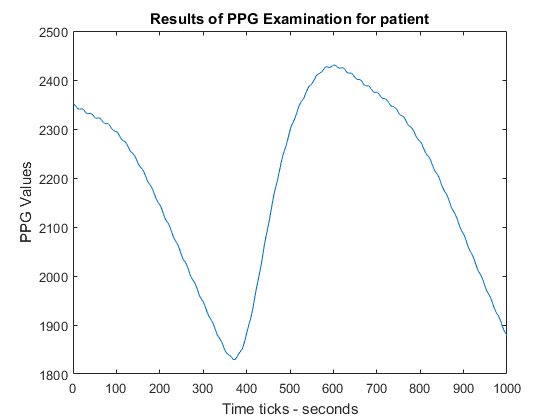
\includegraphics[width=1.4\textwidth,height=10cm]{ppg.png}}\hspace*{-\paperwidth}
\end{figure}

\clearpage
\appendix
\section{Appendix: Script}
\subsection{parser.m}	
{\tt  \lstinputlisting{parser.m}}
\end{document}
